\section{Background}
\label{background}

This section briefly reviews essential background on vehicular security and message authentication codes. 
We assume the reader is familiar with cryptographic hash functions as explained, for example, 
by Stinson~\cite{Stinson} and NIST~\cite{FIPS-180-4}.

%The experienced reader may wish to skip to Section~\ref{problem}. 

	\begin{figure*}
		\centering
		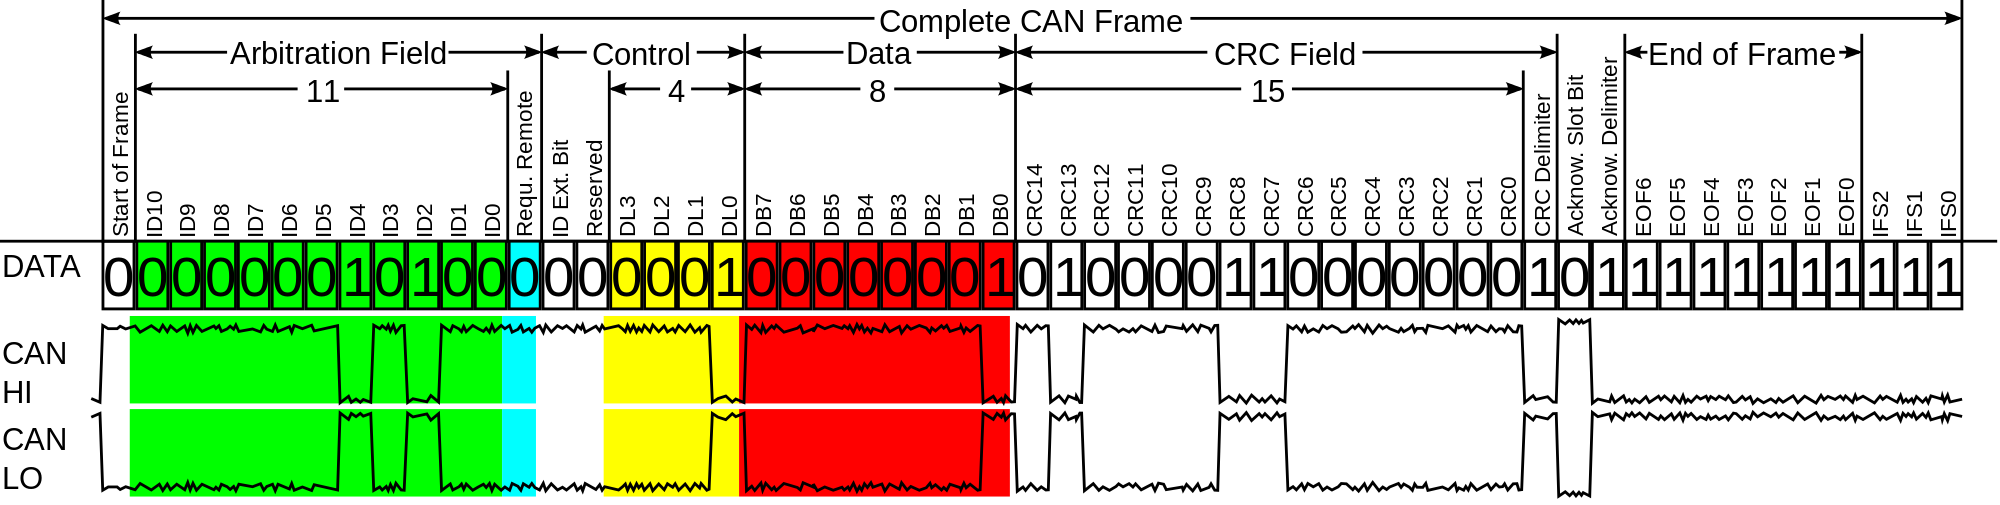
\includegraphics[width=\linewidth]{figures/can_frame.png}
		\caption{The CAN frame~\cite{fig1}.  
		Each transmission on the CAN bus is a structured sequence of 55--111~bits including 8--64 data~bits.}
		\label{fig-frame}
	\end{figure*}

\subsection{ECUs}
\label{ecu}

Electronic Control Units (ECUs) found in an automotive computer network are low-power, single-purpose devices. ECUs on the CAN bus control many components in a modern automobile, from headlights and window controls, to brakes and engine. They are not typically designed with security in mind and frequently comprise a basic CAN bus transceiver, basic message processor, and an actuator. The message processor identifies whether or not a message being broadcast is interesting to the ECU and arbitrates bus rights with the other ECUs. 

\red{Mini-MAC requires write access to nonvolatile memory for full functional operation. Without access to nonvolatile storage, Mini-MAC will still function without full long-term history or stored counters. In this mode, Mini-MAC will still work to authenticate messages, but is less secure than with state-saving capability. Many new ECUs, such as those featuring the TI Hercules series of devices, meet this requirement.}

% give typical chanacteristics (speed, memory)?

\subsection{The CAN Bus}
\label{can}

The Controller Area Network (CAN) bus 
is a simple, low-speed bus designed to network simple nodes. 
It typically runs at 500~kbps in automobiles~\cite{canbus}.\footnote{kilobits per second (kbps).}

Transmissions are organized in frames.  As shown in Figure~\ref{fig-frame}, 
a frame contains an 11-bit identifier field and 
a data payload, as well as some control bits. Figure~\ref{fig-frame} 
shows the allocated data payload space as 8~bits, but
it can be 8 to 64~bits and (based on our observations) is typically 64~bits.
The payload of up to 8~bytes is the most important element, 
as any MAC tag must fit into this frame or use a more complex multi-frame data transmission protocol 
that may or may not be supported on all ECUs. 

We use the term ``message'' to refer to the data payload of one logical transmission.
Any payload longer than 64~bits must be sent as a multi-frame transmission.

To learn more about the characteristics of messages transmitted on the CAN bus, 
the authors captured 15,768 messages from a 2010 Toyota Prius during a 12.27-minute test drive 
around a parking lot on our university campus. 
The drive featured turns, gear changes, reverse driving, and switching on and off 
various instruments and tools including headlights, blinkers, and locks. 

Ideally, and in the case of Mini-MAC, the MAC tag
can fit into the payload together with the data, thus not increasing bus traffic. 
In our test data, 
approximately 61\% of messages contain at most four data bytes
(20\% contain 4~bytes; 16\% contain 3~bytes; 17\% contain 2~bytes; and 8\% contain 1~byte).
Approximately 35\% of messages contain a full 8~data bytes, and 4\% contain 7~bytes.

Thus, for most message, there are at least four bytes of space available for a MAC tag.
Inserting a tag in the unused allocated payload space does not
increase the number of messages sent,
delay any message, 
or increase the number of bits transmitted.

Messages have fixed, known sizes.  The longest messages we witnessed
seemed to be status reports describing the steering wheel angle and tire speed,
with no apparent observable effect on any ECU.
For these long messages with 8-byte payloads,  Mini-MAC will not add a tag. 

We observed approximately 25 messages sent per second on average (40 maximum per second).

\red{Some vehicles use higher-level protocols on top of the CAN protocol to transmit larger messages than CAN can support. Mini-MAC will not break or interfere with these protocols in any way, but we do recommend that any higher-level protocol implement its own message authentication protocol.}

\subsection{Bus Access}
\label{access}

To spoof or replay messages on the CAN bus, the attacker must have access to it.
There are several ways to access the CAN bus:  (1) There is a
physical connection through the On-Board Diagnostic (OBD-II) port, 
typically located underneath the steering wheel.  An attacker might hide
access to this port by splicing into unexposed wires.
(2) An attacker might corrupt an ECU by rewriting its firmware. An attacker might
do so while the car is being serviced or by entering the car while it is parked.
(3) An attacker might gain access to the CAN bus by exploiting or corrupting a peripheral
device connected to it, such as a cellular phone, audio system, or Bluetooth
radio.  For example, Checkoway et al.~\cite{Checkoway-2011} gained bus access by packing 
malware into a WMA audio file played on the car stereo. 
Rouf et al.~\cite{Rouf2010} demonstrated information leakage and message spoofing on RFID-based tire pressure monitoring systems.

Despite many demonstrated security flaws, automotive 
manufacturers have been unreasonably hesitant to acknowledge the vulnerabilities inherent to the CAN bus,
sometimes wishfully claiming that undetected bus access is difficult. 
In 2013, Toyota~\cite{bbc_toyota} offered the following position on automotive security: 
``Toyota has developed very strict and effective firewall technology against such remote and wireless services.'' 
``We believe our systems are robust and secure.'' 
``The presence of a laptop or other device connected to the OBD [on board diagnostics] II port would be apparent.'' 
These statements demonstrate a failure to acknowledge the 
reality of wireless vulnerability of modern vehicles demonstrated in several notable publications.

More recently, insurance companies have begun issuing OBD-II devices 
that track and report driving statistics via cellular modems,
as part of a program to offer more competitive rates to customers. 
The Snapshot tool from Progressive\footnote{www.progressive.com/auto/snapshot/} 
and the Drivewise tool from Allstate\footnote{www.allstate.com/drive-wise.aspx} 
are two examples of these dongles. Foster et al.~\cite{Foster15} 
gained remote access to the CAN bus by hacking these devices.

\subsection{Message Authentication Codes}

Given a message and optionally a key, a Message Authentication Code (MAC) computes a short string (called a tag) 
that a recipient can use, together with the message, to verify the authenticity of the message.  
The recipient, who also knows the key, 
verifies the tag by recomputing it.

The Keyed-Hash Message Authentication Code (HMAC)~\cite{HMAC,FIPS-198-1,rfc2104,nist107} 
is a well-known MAC construction that keys an underlying component hash function.  
Breaking it is as hard as breaking the component hash function.

HMAC is computed as

\begin{equation}
H((k\oplus \text{opad})\concat H((k\oplus \text{ipad})\concat \text{message})) ,
\end{equation}

\noindent
where $k$ is the key, and opad and ipad are the outer and inner hash padding strings, respectively. 
These strings are constant strings defined by 0x5C and 0x36, repeated until the hash input is of the appropriate length. 
$H$ is the component hash function. 
The symbols $\oplus$ and $\concat$ represent exclusive-or (XOR) and concatenation, respectively.

% How much entropy in messages?
% how many key groups?




